\item A particle of mass \( m \) moves in a certain plane \( P \) due to a force \( F \) whose magnitude is constant and whose vector rotates in that plane with a constant angular velocity \( \omega \). Assuming the particle to be stationary at the moment \( t = 0 \), find:
    \begin{center}
        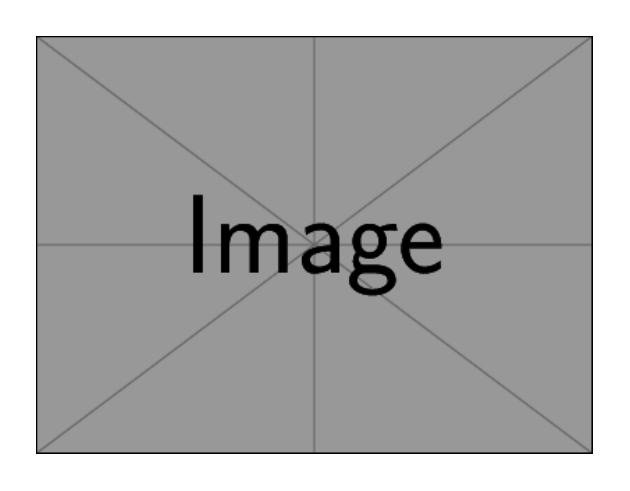
\begin{tikzpicture}
            \node at (0, 0) {\includegraphics[scale=0.5]{example-image.png}};
        \end{tikzpicture}
    \end{center}
    \begin{enumerate}
        \item its velocity as a function of time;
        \item the distance covered by the particle between two successive stops, and the mean velocity over this time.
    \end{enumerate}